% !TEX root = ../thesis.tex

\documentclass[thesis.tex]{subfiles}


\begin{document}

\chapter{Introduction}
\label{chapter:intro}


% http://ipimediaworld.com/wp-content/uploads/2013/10/Turning-your-smartphone.pdf

\sout{Tsekkaa löytyskö LuminoTrace PowerPointista vielä jotain pointteja?
Aiheen rajaus johdantoon.
Johdanto selvittaa samat asiat kuin tiivistelma, mutta laveammin. Johdannossa kerrotaan yleensa seuraavat asiat
Kuten kirjallisessa osassa todettiin, vaarentajat pyrkivat selvittamaan tekniikan periaatteen nopeasti, joten turvallisuussovelluksissa kaytettavia merkintoja on oltava riittavan monimutkaisia ja niita on voitava muunnella helposti. Kuten luvuissa 2.1.1-2.1.2 todettiin, luminoforien luminesenssiominaisuudet muuttuvat yhdisteen rakenteen muuttuessa. Erilaisten rakenteiden suunnitelmallinen synteesi onkin tarkeaa, mikali tekniikkaa halutaan kehittaa eteenpain. Luminoforien viritys- ja emissioaallonpituuksien tulisi soveltua myos kaytetyn laitteiston vaatimuksiin.
Fotoluminesenssiin perustuva pintamerkkiaineteknologia}

\begin{itemize}
\item[--]Tutkimuksen taustaa ja tutkimusaiheen yleisluonteinen esittely
\item[--]Tutkimuksen tavoitteet
\item[--]Paakysymys ja osaongelmat
\item[--]Tutkimuksen rajaus ja keskeiset kasitteet
\end{itemize}

\sout{Product authentication, or brand protection, ...
This thesis explores an alternative, competing technology.
The focus of this thesis is the design and implementation of a scalable hybrid mobile application. The application will be developed as a part of the LuminoTrace project at Aalto CHEM for the purposes production authenticaion.
The verification is done by analyzing the spectrum of a special chemical compound embedded in the material. Both the underlying algorithm and the compound have already been developed as a part of the LuminoTrace project.}

\sout{The functionality outlined above can be largely achieved by utilizing existing Web technologies. However, a more granular control over the camera (e.g. burst-mode, flash settings) will require a native component to be implemented for each target platform. The preliminary target platform will be Windows Phone (WP). To improve scalability the fingerprint will be computed on the client-side. This will require for the existing algorithm to be ported into JavaScript. Scalability can be further improved by offloading parts of the (fingerprint) database from the server to the user's device.}

%Moreover, usability is improved as the application can function offline without the overhead of network latency. Hosting fingerprint data on the user's device might however have security implications: can the data be safely/efficiently encrypted on the user's device? The product authentication ecosystem \ref{fig:landscape}.

\begin{figure}[h!]
\centering 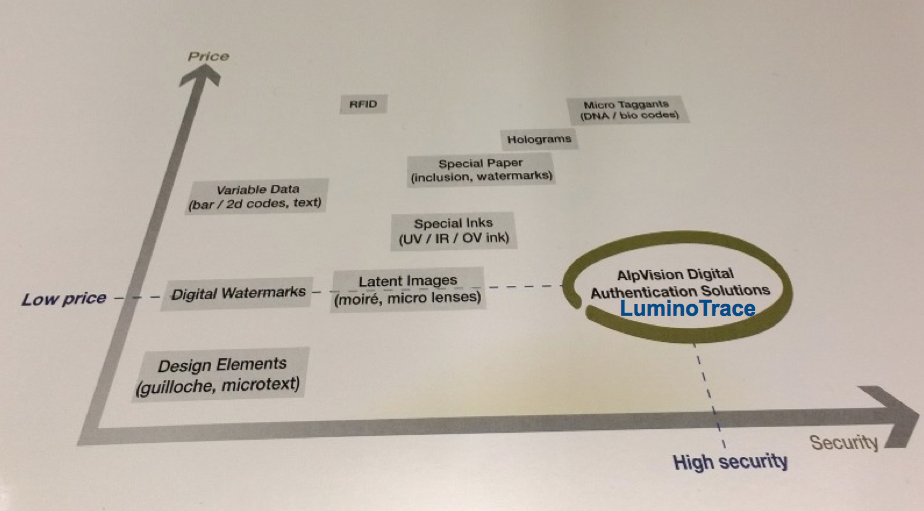
\includegraphics[width=\linewidth]{images/landscape}
\caption{Product authentication landscape \label{fig:landscape}}
\end{figure}

\section{Research Questions}
\label{chapter:research-questions}

This thesis aims to answer the following questions:

\begin{itemize}
  \item \label{RQ1} \textbf{RQ1}: How can photoluminescence and smartphones be integrated for product authentication purposes?
  \item \label{RQ2} \textbf{RQ2}: Which factors affect the analysis of photoluminescent material (luminophores) in the context of smartphones?
  \item \label{RQ3} \textbf{RQ3}: Does modern smartphone technology provide the means for photoluminescence based product authentication in practice?
\end{itemize}


\end{document}